\documentclass[pdftex,12pt,xcolor=svgnames]{beamer}

\mode<presentation>
{
  \usetheme{boxes}
  \usecolortheme[named=MidnightBlue]{structure}
  %\setbeamercolor{normal text}{bg=NavajoWhite!20}
  %% \usefonttheme{serif}
  \setbeamertemplate{navigation symbols}{}
  % Show frame number and author name in footline
  \setbeamertemplate{frametitle}[default][center]
  \setbeamertemplate{footline}[frame number]
  \setbeamertemplate{items}[circle]
  %\addtobeamertemplate{footline}{\quad\textcolor{gray}{James Robert Lloyd}}{}
  % Set frame titles in small capitals
  %% \setbeamerfont{frametitle}{shape=\scshape,family=\rmfamily,size={\fontsize{16}{20}}}
  %% \setbeamercolor{frametitle}{bg=gray!60!white,fg=black}
  %% \setbeamercolor{frametitle}{bg=blue,fg=black}
  % Alerted text: blue (uncomment second line if theme sets alerted text to bold)
  \setbeamercolor{alerted text}{fg=blue}
  %\setbeamerfont*{alerted text}{}
  \setbeamertemplate{bibliography item}[text] %{\hbox{\donotcoloroutermaths$\blacktriangleright$}}
  \setbeamertemplate{bibliography entry title}{}
  \setbeamertemplate{bibliography entry author}{}
  \setbeamertemplate{bibliography entry note}{}
  \setbeamertemplate{bibliography entry location}{}

}
\usepackage[english]{babel}
\usepackage[latin1]{inputenc}
\usepackage{times}
\usepackage[T1]{fontenc}
\usepackage{hyperref}
\usepackage{multimedia}
\usepackage{eepic}
\usepackage{graphicx}
%\usepackage[nohug]{latexinclude/diagrams}
\usepackage{tikz}
\usetikzlibrary{calc}

%% \newcommand{\footlineextra}[1]{
%%     \begin{tikzpicture}[remember picture,overlay]
%%         \node[yshift=1.5ex,anchor=south east] at (current page.south east)
%% {#1};
%%     \end{tikzpicture}
%% }

\newcommand{\footlineextra}[1]{
    \begin{tikzpicture}[remember picture,overlay]
        \node[xshift=-5ex,yshift=-0.5ex,anchor=south east] at (current page.south east)
             {\mbox{\tiny \textcolor{MidnightBlue}{#1}}};
    \end{tikzpicture}
}

\def\sectionframe#1{
  {
    \setbeamertemplate{footline}{\empty}
    \begin{frame}{}
      \begin{center}
        \huge\sc #1
      \end{center}
    \end{frame}
  }
}


\usepackage{etex}
\usepackage{tabularx}
\usepackage{include/picins}
\usepackage{include/preamble}
\usepackage{setspace}
\usepackage{xcolor}
\usepackage{tikz}
\usepackage{listings}
%\usepackage{algorithm}
%\usepackage{algpseudocode}

\definecolor{Blue}{rgb}{0.0,0.0,1.0}
\lstloadlanguages{Python}%
\lstset{language=Python,
        frame=none,
        basicstyle=\tiny\ttfamily\bfseries,
        keywordstyle=[1]\color{Blue},
        keywordstyle=[2]\color{Purple},
        commentstyle=\usefont{T1}{pcr}{m}{sl}\color{Green},
        keepspaces=true,
        }
\lstset{language=Python} 

\newcommand{\params}{\vx}
\newcommand{\learnrate}{\alpha}
\newcommand{\decay}{\beta}

\setlength{\columnsep}{0.03\textwidth}
\setlength{\columnseprule}{0.0018\textwidth}
\setlength{\parindent}{0.0cm}
\hypersetup{colorlinks=true,citecolor=blue}
\newcommand{\paren}[1]{\left( #1 \right)}
\newcommand{\vv}{\mathbf{v}}

\title{Hyperparameter optimization: \\ Why not use gradients?}
%\title{Gradient-based Hyperparameter Optimization with Reversible Learning}

\author{
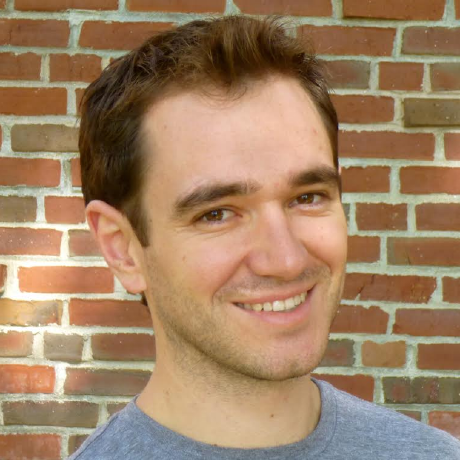
\includegraphics[height=0.16\textwidth]{talkfigs/dougal}
\qquad\qquad
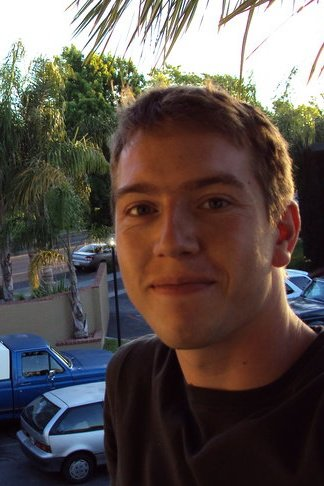
\includegraphics[height=0.16\textwidth, trim=20mm 25mm 0mm 25mm, clip]{talkfigs/david2}
\qquad\qquad
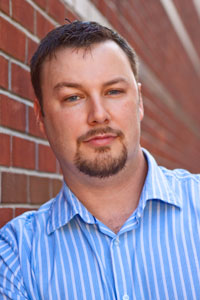
\includegraphics[height=0.16\textwidth]{talkfigs/adams}
\\
Dougal Maclaurin, David Duvenaud, Ryan Adams}

%\institute{Harvard University}
\institute{
\includegraphics[height=0.16\textwidth]{talkfigs/harvard.jpg}}


\date{}

\begin{document}

\frame[plain] {\titlepage}

\frame[plain]{
\frametitle{Motivation}
\begin{itemize} 
  \item Hyperparameters are everywhere
  \begin{itemize}
	\item sometimes hidden
  \end{itemize}
  \item Gradient-free optimization hard in high dimensions
  \item Validation loss is a function of hyperparameters
  \item Why not take gradients?
\end{itemize}}

\frame[plain]{\frametitle{Optimizing optimization}
\center ${\params_{final} = \textnormal{SGD} \left(\params_{init}, \textnormal{learn rate}, \textnormal{momentum}, \textnormal{Loss}(\params, \textnormal{reg}, Data) \right)}$

\includegraphics<1>[width=0.9\columnwidth]{talkfigs/learning_curves_1.pdf}
\includegraphics<2>[width=0.9\columnwidth]{talkfigs/learning_curves_2.pdf}
\includegraphics<3>[width=0.9\columnwidth]{talkfigs/learning_curves_3.pdf}
}



\frame[plain]{\frametitle{A closer look}
\center ${J = Loss \left( D_{val}, \textnormal{SGD} \left(\vw_{init}, \learnrate, \decay, \textnormal{Loss}(D_{train}, \vw, \textnormal{reg}) \right)\right)}$

\center ${\frac{\partial J}{\partial D_{train}} = Loss \left( D_{val}, \textnormal{SGD} \left(\vw_{init}, \learnrate, \decay, \textnormal{Loss}(D_{train}, \vw, \textnormal{reg}) \right)\right)}$
}


\frame[plain]{\frametitle{Technical Challenge: Memory}
\begin{itemize}
\item Reverse-mode differentiation needs access to entire learning trajectory
\item i.e.\ $10^7$ parameters $\times$ $10^5$ training iterations
\item Only need access in reverse order...
\item Could we recompute the learning trajectory backwards by running reverse SGD?
\end{itemize}}

\frame[plain]{\frametitle{SGD with momentum is reversible}
Forward update rule:
\begin{align*}
\vx_{t+1} & \leftarrow \vx_t + \alpha \vv_t \\
\vv_{t+1} & \leftarrow \beta \vv_t - \nabla L\left(\vx_{t+1}\right)
\end{align*}
Reverse update rule:
\begin{align*}
\vv_{t} & \leftarrow \left(\vv_{t+1} + \nabla L\left(\vx_{t+1}\right)\right)/\beta \\
\vx_{t} & \leftarrow \vx_{t+1} - \alpha \vv_t
\end{align*}
}

\frame[plain]{\frametitle{Naive reversal \phantom{... Fails!}}
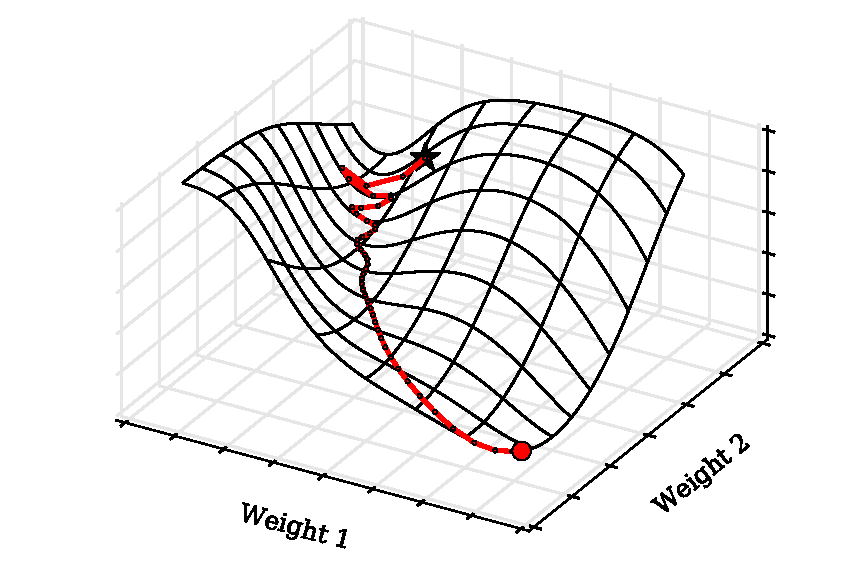
\includegraphics[width=0.9\columnwidth]{../experiments/Jan_25_Figure_1/4_naive_reverse/learning_curve_forward.pdf}}

\frame[plain]{\frametitle{Naive reversal ... Fails!}
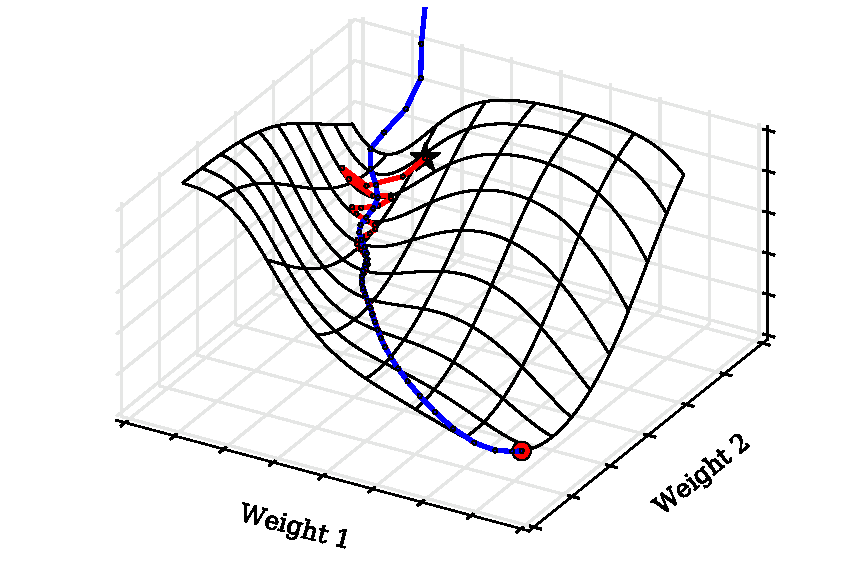
\includegraphics[width=0.9\columnwidth]{../experiments/Jan_25_Figure_1/4_naive_reverse/learning_curve_reverse.pdf}}

\frame[plain]{\frametitle{A closer look at reverse SGD}
Forward update rule:
\begin{align*}
\vx_{t+1} & \leftarrow \vx_t + \alpha \vv_t \\
\vv_{t+1} & \leftarrow \beta \vv_t - \nabla L\left(\vx_{t+1}\right)
\end{align*}
%\begin{itemize}
%\item 
Destroys $\log_2 \beta$ bits per parameter per iteration 
%\end{itemize}

\vspace{1cm}

Reverse update rule:
\begin{align*}
\vv_{t} & \leftarrow \left(\vv_{t+1} + \nabla L\left(\vx_{t+1}\right)\right)/\beta \\
\vx_{t} & \leftarrow \vx_{t+1} - \alpha \vv_t
\end{align*}
%\pause
%\begin{itemize}
%\item 
Needs $\log_2 \beta$ bits per parameter per iteration 
%\end{itemize}

}

\lstset{basicstyle=\small\ttfamily\bfseries}

\frame[plain]{\frametitle{How to store the lost bits?}
\begin{itemize} 
\item Switch to fixed-precision for exact addition
\item Express $\beta$ as a rational number
\item push/pop remainders from an information buffer
\end{itemize}
%\item Information buffer can use any LIFO coding method
\lstinputlisting{code/infobuffer.py}
\begin{itemize} 
\item 200X memory savings when $\beta = 0.9$
\end{itemize}
}


\frame[plain]{\frametitle{Learning rate gradients}
\begin{columns}
\begin{column}{6cm}
\begin{align*}
\frac{\partial Loss \left( D_{val}, \params_{init}, \learnrate, \decay, D_{train}, \textnormal{reg} \right)}{\partial \learnrate}
\end{align*} 
\end{column}
\begin{column}{4cm}
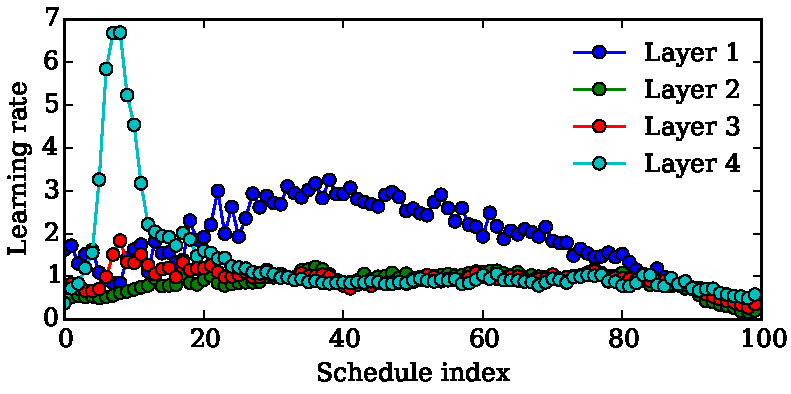
\includegraphics[width=0.6\columnwidth, clip, trim=9cm 3cm 0.8cm 0.5cm]{../experiments/Feb_3_training_schedules/3_adam_50/schedules_small.pdf}
\end{column}
\end{columns}

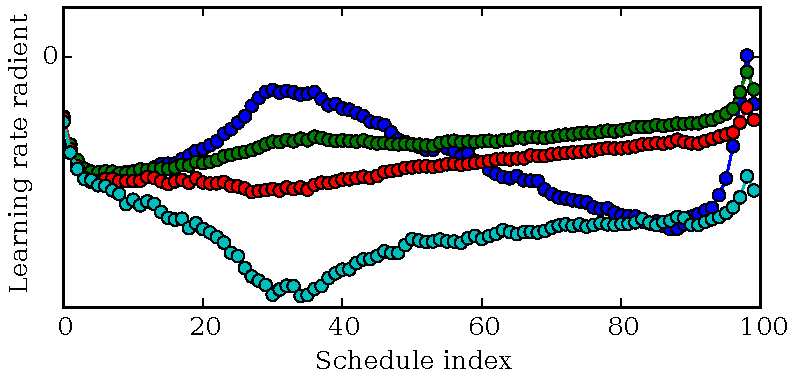
\includegraphics[width=\columnwidth]{../experiments/Feb_3_training_schedules/5_initial_gradient/schedules_small.pdf}
}

\frame[plain]{\frametitle{Optimized learning rates}
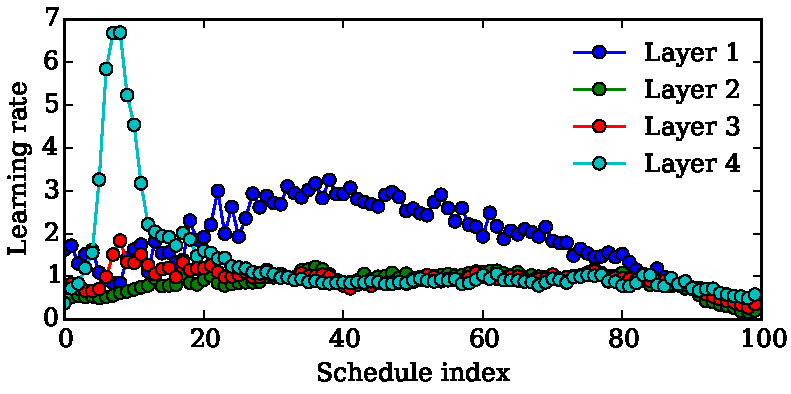
\includegraphics[width=\columnwidth]{../experiments/Feb_3_training_schedules/3_adam_50/schedules_small.pdf}}

\frame[plain]{\frametitle{Optimizing initialization scales} 
\begin{center}
\begin{align*}
\frac{\partial Loss \left( D_{val}, \params_{init}, \learnrate, \decay, D_{train}, \textnormal{reg} \right)}{\partial \params_{init}}
\end{align*}
\begin{tabular}{cc}
 Biases & Weights \\
\hspace{-1em}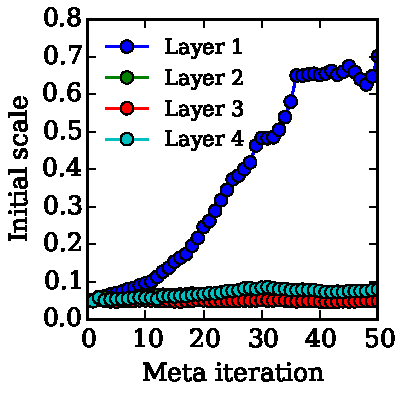
\includegraphics[width=0.5\columnwidth, height=0.5\columnwidth]{../experiments/Feb_3_training_schedules/3_adam_50/init_bias_learning_curve.pdf} &
\hspace{-1em}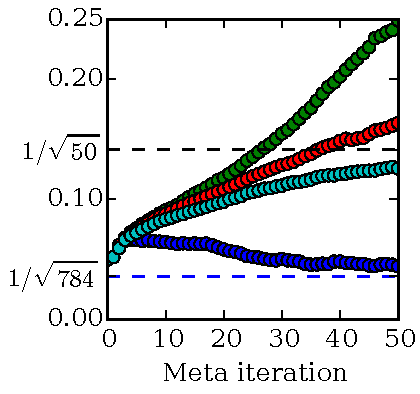
\includegraphics[width=0.5\columnwidth, height=0.5\columnwidth]{../experiments/Feb_3_training_schedules/3_adam_50/init_weight_learning_curve.pdf}
\end{tabular}
\end{center}}

\frame[plain]{\frametitle{Optimizing regularization}
\center
\begin{align*}
\frac{\partial Loss \left( D_{val}, \params_{init}, \learnrate, \decay, D_{train}, \textnormal{reg} \right)}{\partial \textnormal{reg}}
\end{align*}
Optimized $L_2$ regularization hyperparameters for each weight in a logistic regression  trained on MNIST.
\vspace{0.5in}
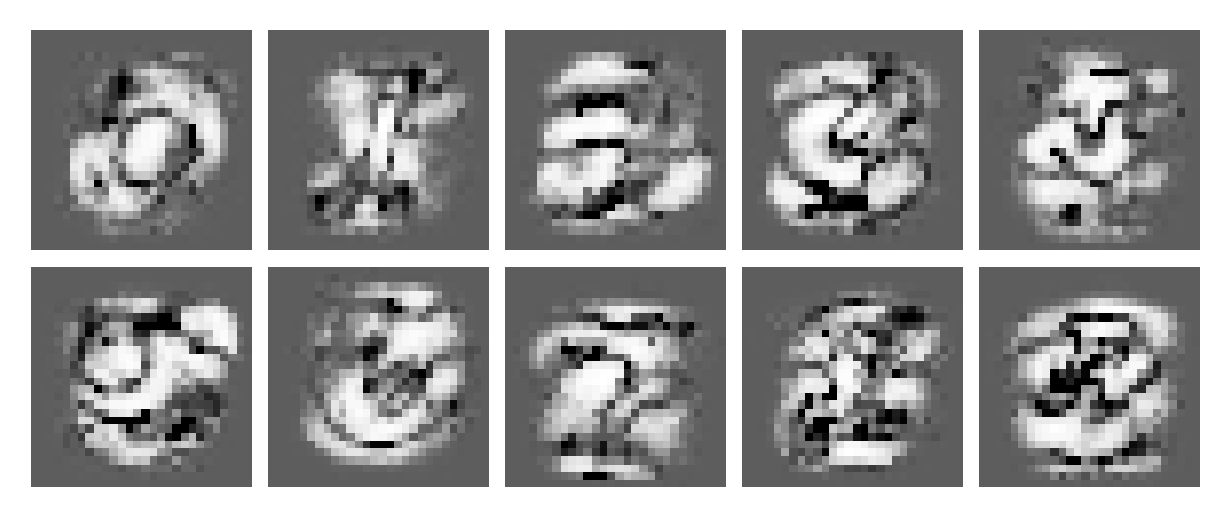
\includegraphics[width=\columnwidth]{../experiments/Jan_21_nn_ard/2/penalties.pdf}
}

\frame[plain]{\frametitle{Optimizing architecture}
\begin{center}
\begin{itemize} 
  \item Architecture is regularization
  \item Regularization can be continuous
  \item Continuous functions can be differentiated
  \item Could generalize convnets, recurrent nets, multi-task
\end{itemize}
\vspace{1cm}
\begin{columns}
\begin{column}{5.5cm}
\begin{tabular}{cc}
\hspace{-3mm}\rotatebox{90}{\tiny{ \qquad Rotated \qquad \quad Original}} & 
\hspace{-3mm}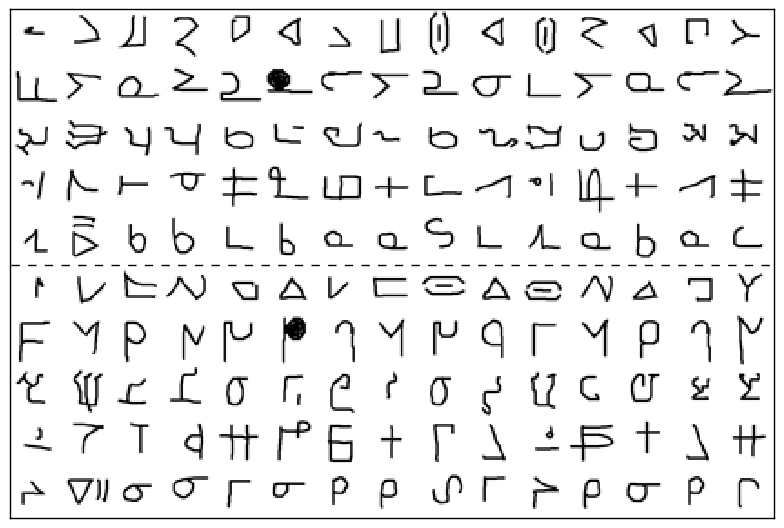
\includegraphics[width=0.85\columnwidth]{../experiments/Feb_4_augmented_omniglot/2_rotated_90/all_alphabets.png}
\end{tabular}
\end{column}
\begin{column}{5cm}
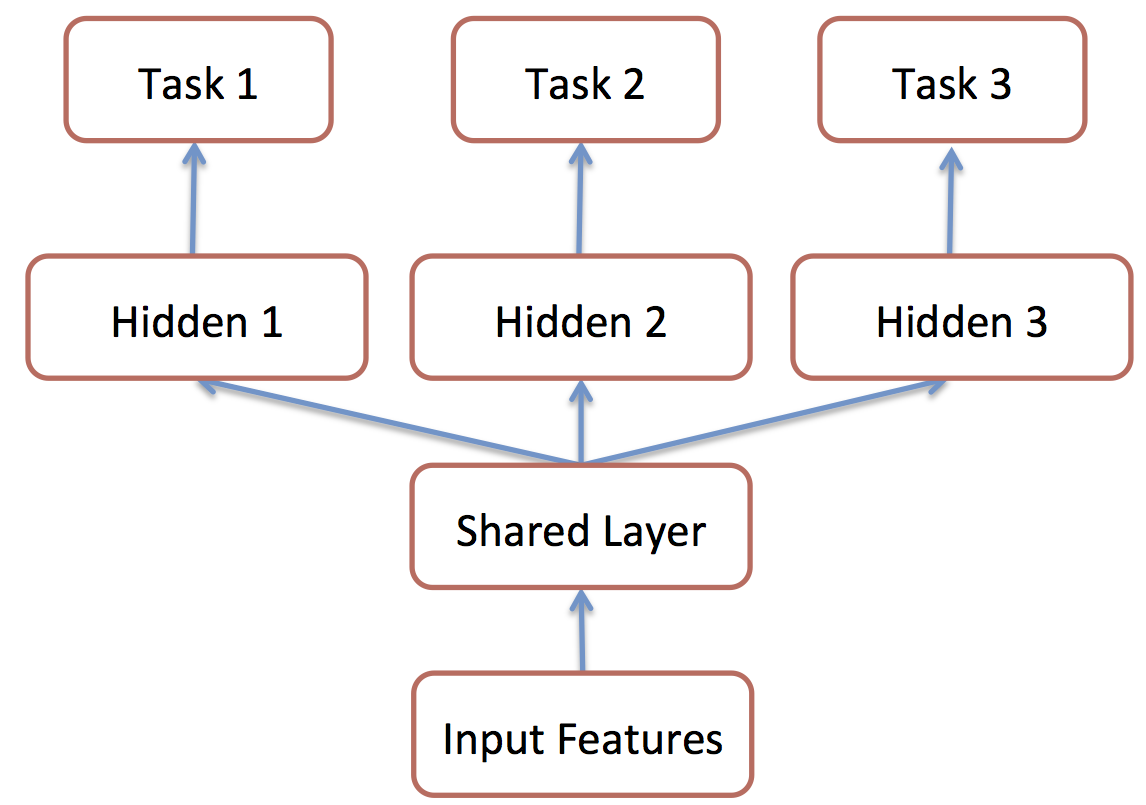
\includegraphics[width=\columnwidth]{talkfigs/shared-net.png}
\end{column}
\end{columns}
\end{center}}

\newcommand{\omniimagea}[2]{\parbox{4em}{\includegraphics[width=1.4cm]{../experiments/Feb_4_augmented_omniglot/2_rotated_90/minifigs/learned_corr_#1_#2.pdf}}}%
\newcommand{\omniimageb}[1]{\omniimagea{#1}{0} & \omniimagea{#1}{1} & \omniimagea{#1}{2}}%

\frame[plain]{\frametitle{Optimizing regularization}
\begin{center}
\begin{tabular}{c@{\hskip 0.9em}ccc@{\hskip 0.9em}c@{\hskip 0.9em}c}%
\renewcommand{\tabcolsep}{1pt}
& Input   & Middle  & Output & Train & Test\\
& weights & weights & weights & error & error \\
\parbox{3.7em}{Separate networks} & \omniimageb{no_sharing}      & 0.61 & 1.34\\ \hline
\parbox{3.7em}{Tied weights}      & \omniimageb{full_sharing}    & 0.90 & 1.25\\ \hline
\parbox{3.7em}{Learned sharing}   & \omniimageb{learned_sharing} & 0.60 & \bf 1.13
\end{tabular}
\end{center}}

\frame[plain]{\frametitle{Optimizing training data}
\center
\begin{align*}
\frac{\partial Loss \left( D_{val}, \params_{init}, \learnrate, \decay, D_{train}, \textnormal{reg} \right)}{\partial D_{train}}
\end{align*}
\vspace{0.5in}
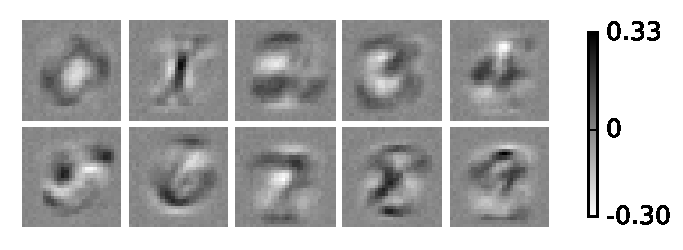
\includegraphics[width=\columnwidth]{../experiments/Jan_19_optimize_data/9_color_bar/fake_data.pdf}
}

\frame[plain]{\frametitle{Limitations: Chaotic learning dynamics}
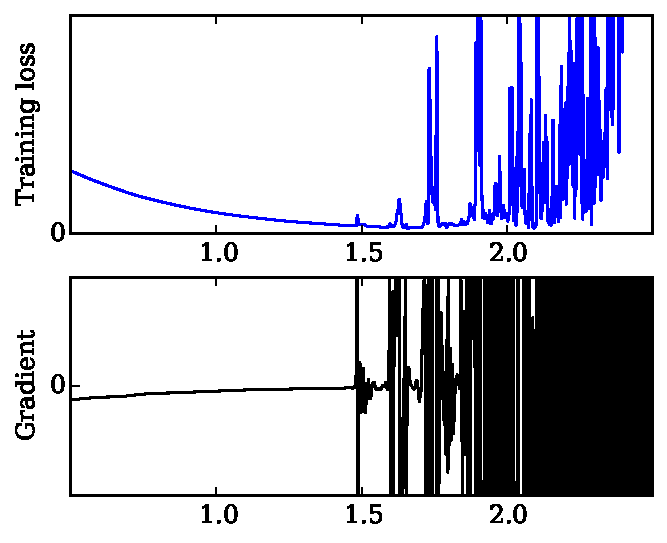
\includegraphics[width=0.9\columnwidth]{../experiments/Jan_14_learning_rate_wiggliness/3/chaos.pdf}
\vspace{-1.6em}
\center Learning rate}



\frame[plain]{\frametitle{Autograd: Automatic Differentiation} 
\begin{itemize} 
  \item \url{github.com/HIPS/autograd}
  \item Simple ($\sim$ 300 lines of code)
  \item Functional interface
  \item Works with (almost) arbitrary Python/Numpy code
  \item Can take gradients of gradients (of gradients...)
\end{itemize}}

\frame[plain]{\frametitle{Autograd Examples}
\begin{columns}
\begin{column}{5.5cm}
\lstinputlisting{code/sinusoid.py} 
\end{column}
\begin{column}{5cm}
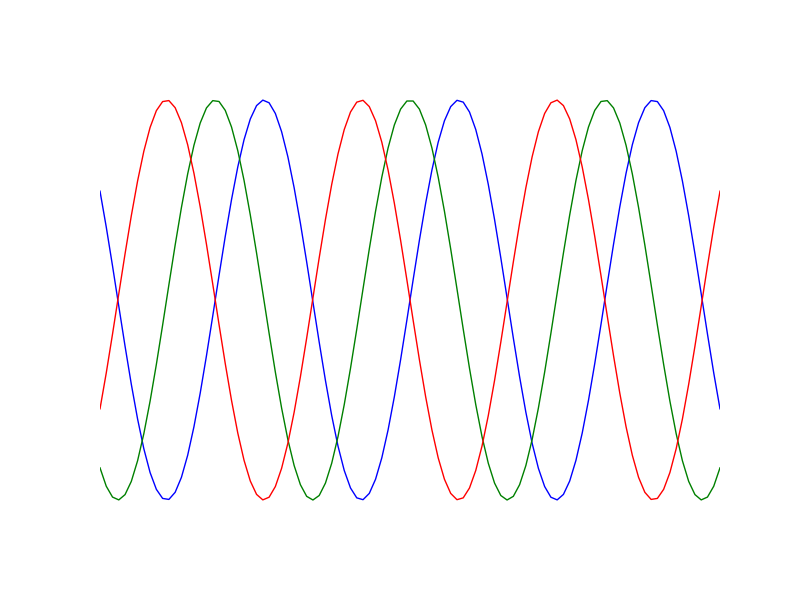
\includegraphics[width=6cm]{code/sinusoid.png}
\end{column}
\end{columns}}

\frame[plain]{\frametitle{Autograd Examples}
\begin{columns}
\begin{column}{5.5cm}
\lstinputlisting{code/sinusoid-taylor.py} 
\end{column}
\begin{column}{5cm}
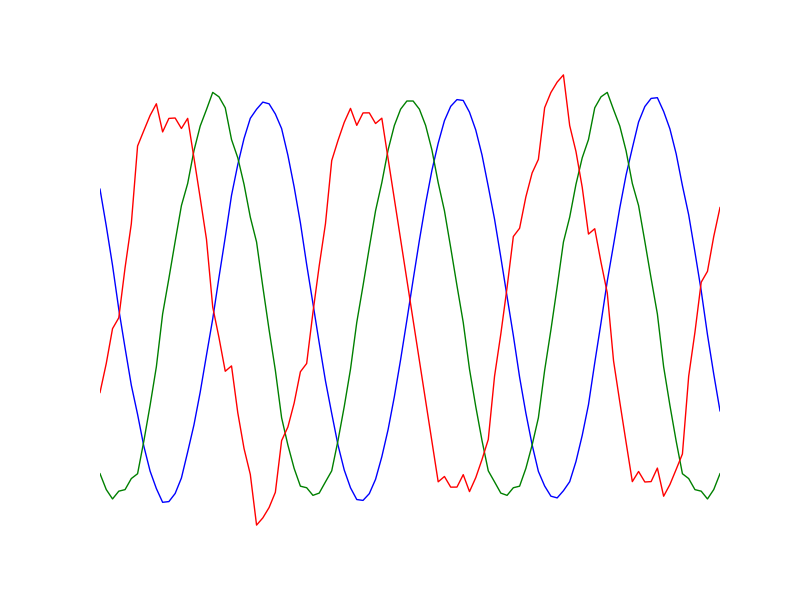
\includegraphics[width=6cm]{code/sinusoid_taylor.png}
\end{column}
\end{columns}}

\frame[plain]{\frametitle{Autograd Examples}
\begin{columns}
\begin{column}{5.5cm}
\lstinputlisting{code/tanh.py}
\end{column}
\begin{column}{5cm}
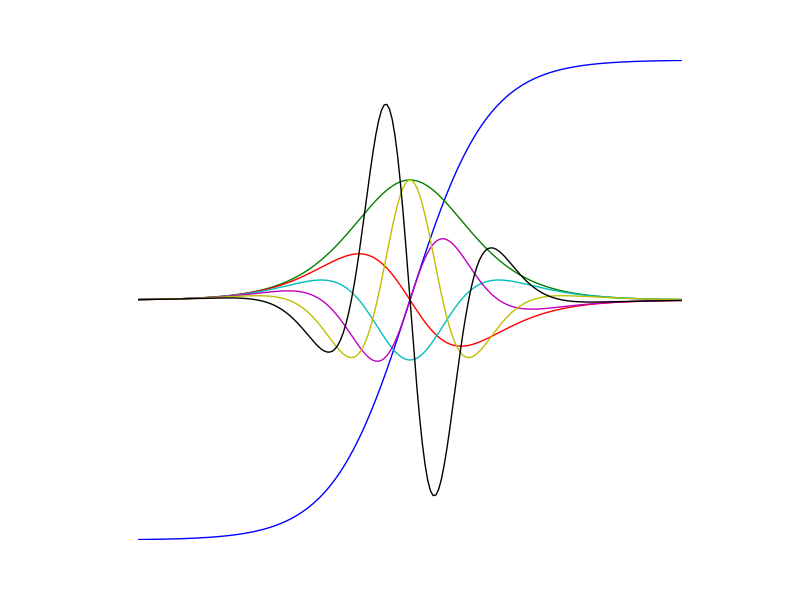
\includegraphics[width=6cm]{code/tanh.png}
\end{column}
\end{columns}}

\frame[plain]{\frametitle{Most Numpy functions implemented}

\vspace{0.5cm}

\newcommand{\us}{\textunderscore}
\centerline{
\begin{tabular}{llllllll}
 Complex             & Array         & Misc      & Linear   & Stats   \\
 \& Fourier          &               &           & Algebra  &          \\
\midrule
 imag                & atleast\us 1d & logsumexp & inv      & std      \\
 conjugate           & atleast\us 2d & where     & norm     & mean  \\
 angle               & atleast\us 3d & einsum    & det      & var   \\
 real\us if\us close & full          & sort      & eigh     & prod     \\
 real                & repeat        & partition & solve    & sum       \\
 fabs                & split         & clip      & trace    & cumsum  \\
 fft                 & concatenate   & outer     & diag     &        \\
 fftshift            & roll          & dot       & tril     &         \\
 fft2                & transpose     & tensordot & triu     &        \\
 ifftn               & reshape       & rot90     &          &        \\
 ifftshift           & squeeze       &           &          &        \\
 ifft2               & ravel         &           &          &        \\
 ifft                & expand\us dims&           &          &        \\
 fftn                & flipud        &           &          &        \\
                     & fliplr        &           &          &        \\
\end{tabular}}
}


%% \frame[plain]{\frametitle{Other possible applications}} % DM
\frame[plain]{\frametitle{Summary}
\begin{itemize}
\item Can compute gradients of learning procedures
\item Reversing learning saves memory
\item Can optimize thousands of hyperparameters
%\item There is a deep connection between learning and entropy
\end{itemize}

\pause
\centerline{Thanks!}
}

\end{document}

\frame[plain]{\frametitle{Entropy and Optimization are Duals}
\centerline{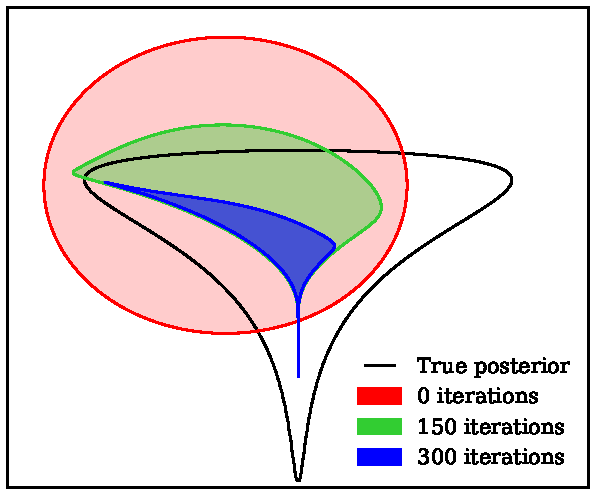
\includegraphics[width=0.9\columnwidth]{talkfigs/dists}}}


\frame[plain]{\frametitle{Reverse-mode Differentiation}
\begin{align*}
\onslide<1->{\pderiv{}{x} L\paren{F\paren{G\paren{H\paren{x}}}}
             & = \pderiv{L}{F}\pderiv{F}{G}\pderiv{G}{H}\pderiv{H}{x} \\}
\onslide<2->{& = \pderiv{L}{F}\paren{\pderiv{F}{G}\paren{\pderiv{G}{H}\pderiv{H}{x}}} %\quad &\text{Forward mode}
\\
             & = \paren{\paren{\pderiv{L}{F}\pderiv{F}{G}}\pderiv{G}{H}}\pderiv{H}{x} %\quad &\text{Reverse mode}
             }
\end{align*}
\onslide<3>{
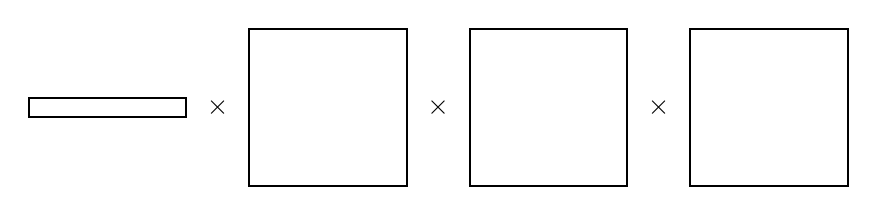
\begin{tikzpicture}[thick, scale=0.4]
  \draw (1,3.2) rectangle (6, 3.8);
  \draw (8,1) rectangle (13, 6);
  \draw (15,1) rectangle (20, 6);
  \draw (22,1) rectangle (27, 6);
  \node at (7, 3.5) {$\times$};
  \node at (14, 3.5) {$\times$};
  \node at (21, 3.5) {$\times$};
\end{tikzpicture}}
}


